% !TEX root = ../../../main.tex
% 来源：高中物理甲种本·第三册（电磁·光学·近代物理）
% 章节：交流电 / 表征交流电的物理量
% 原始文件：3.tex，行 297-311
% 类型：tikz
% ---
    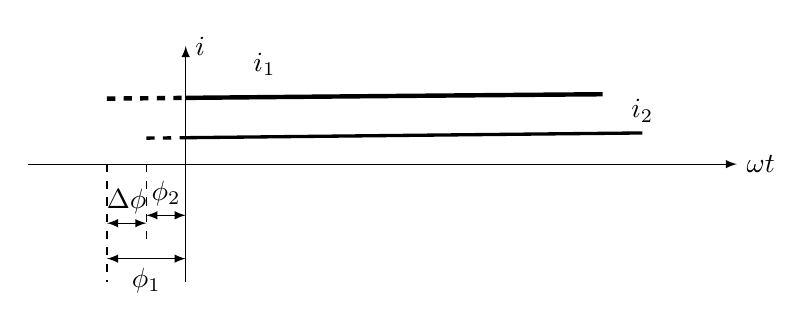
\begin{tikzpicture}[>=latex, xscale=1]
        \draw [->](-2,0)--(7,0)node[right]{$\omega t$};
        \draw [->](0,-1.5)--(0,1.5)node[right]{$i$};
        \draw [ultra thick] plot[domain=0:5.3, samples=1000, variable=\x] (\x, {sin(\x+1 r)}) ;
        \draw [ultra thick, dashed] plot[domain=-1:0, samples=100, variable=\x] (\x, {sin(\x+1 r)});
        \node at (1,1) [above]{$i_1$};
        \draw [very thick] plot[domain=0:5.3+.5, samples=1000, variable=\x] (\x, {.7*sin(\x+.5 r)})node [above]{$i_2$} ;
        \draw [very thick, dashed] plot[domain=-.5:0, samples=100, variable=\x] (\x, {.7*sin(\x+.5 r)});
        \draw [dashed] (-1,0)--(-1,-1.5);\draw [dashed] (-.5,0)--(-.5,-1);
        \draw [<->] (0,-1.2)--node[below]{$\phi_1$}(-1, -1.2);
        \draw [<->] (0,-.65)--node[above]{$\phi_2$}(-.5,-.65);
        \draw [<->] (-1,-.75)--node[above]{$\Delta \phi$}(-.5,-.75);


\end{tikzpicture}
